\chapter[O Estudo de Caso]{O Estudo de Caso}

Neste capítulo será apresentado o estudo de caso desse trabalho. Na primeira seção será apresentado o contexto e a caracterização da organização do estudo de caso. Na segunda seção será apresentada a empresa contratada para o desenvolvimento do projeto. Na terceira seção será apresentada a caracterização do contrato e o objeto do contrato, ou seja, a caracterização do projeto que os dados foram coletados. Na quarta seção será apresentada a solução aplicada na gestão do contrato analisado. E, finalmente, na quinta seção serão apresentadas a análise dos dados e a discussão dos resultados.

\section[A Organização]{A Organização}

O órgão escolhido, IPHAN, possui uma força de trabalho atuante na área de TI de apenas 8 funcionários, dos quais apenas 4 trabalham diretamente com sistemas. O perfil dessa equipe é apresentado na Tab. (2). Devido ao número reduzido de servidores disponíveis na área de TI do órgão, frequentemente uma mesma pessoa acaba desempenhando diferentes papeis requeridos pela Instrução Normativa MP/SLTI Nº04/2010.

\begin{table}[H]
\center
\footnotesize
\begin{tabular}{|c|c|c|}
\hline
\textbf{Área}          & \textbf{Perfil}   & \textbf{Quantidade} \\ \hline
TI Geral               & Coordenador de Tecnologia da Informação   & 1                   \\ \hline
Infraestrutura         & Analista de Tecnologia da Informação do MP   & 2                   \\ \hline
Sistemas               & Analista de Tecnologia da Informação do MP   & 2                   \\ \hline
\multirow{3}{*}{Apoio} & Analista de Tecnologia da Informação do MP   & 1                   \\ \cline{2-3} 
\multicolumn{1}{|l|}{} & Servidor do Ministério da Ciência, Tecnologia e Inovação & 1                   \\ \cline{2-3} 
\multicolumn{1}{|l|}{} & Servidor do IPHAN & 1                   \\ \hline
\end{tabular}
\caption{Perfil da Equipe do IPHAN}
\end{table}

O contexto atual do órgão foi identificado por meio da aplicação da técnica de entrevista informal, de questionário e da documentação disponível do órgão. O questionário aplicado pode ser encontrado no Apêndice I - Questionário Gestão do Contrado. Vale ressaltar que esse questionário foi aplicado não só para caracterização da organização como também para coleta de dados quantitativos necessários para o estudo de caso deste trabalho e ele foi projetado de forma generalizada para que tanto o IPHAN quanto a empresa contratada, EGL - Engenharia, pudessem respondê-lo.
 
Os fatores mais significantes que são gerenciados pela área de TI do órgão são:
\begin{itemize}
\item Atender as demandas para desenvolvimento de sistemas (sistema novo, manutenção, documentação).
\item Controlar de qualidade de sistemas.
\item Possuir medições de sistemas.
\end{itemize}

Por meio do questionário foram identificados fatores que motivaram o uso de métodos ágeis na gestão do contrato do órgão.A Tab. (3) mostra a porcentagem dos fatores motivacionais citados pelos servidores da área de sistemas do órgão. 

\begin{table}[H]
\center
\footnotesize
\begin{tabular}{|c|c|}
\hline
\textbf{Fator Motivacional}          & \textbf{Porcentagem}  \\ \hline
Documentação desnecessária estava \\ sendo produzida e entregue               &  100\%                 \\ \hline
Entrega de software funcional era pouco \\ frequente nos contratos anteriores        &  66\%                  \\ \hline
Visibilidade do processo era baixa              &  66\%                \\ \hline
O fiscal técnico do contrato e o gestor do \\ contrato não estavam exercendo os seus papéis como deveriam              &  66\%                \\ \hline
A satisfação do cliente era baixa              &  66\%                \\ \hline
Visibilidade do processo era baixa              &  66\%                \\ \hline
A qualidade do produto era preocupante   &  66\%                \\ \hline
Os requisitos de software não eram atendidos &  66\%                \\ \hline
\end{tabular}
\caption{Fatores motivacionais}
\end{table}


No que diz respeito a aplicação de métodos ágeis na gestão do contrato, de acordo com a Instrução Normativa MP/SLTI Nº04/2010, a fase de Gerenciamento de Contrato deve conter as seguintes etapas: início do contrato; encaminhamento formal de ordem de serviço ou fornecimento de bens  monitoramento da execução; e transição contratual e/ou encerramento do contrato. Todas estas etapas foram contempladas no processo definido pelo órgão, fazendo com que ele seja aderente ao normativo e adequado para o estudo de caso deste trabalho.

As metas norteadoras para a elaboração do processo de gestão de contrato com métodos ágeis foram:
\begin{itemize}
\item Ser aderente à legislação pertinente;
\item Entregar \textit{software} mais rapidamente;
\item Focar na gestão do contrato e na definição de uma metodologia de gestão de demandas;
\item Não focar em dizer como a empresa deveria desenvolver o \textit{software}, ou seja, não definir metodologia de desenvolvimento de \textit{software};
\item Satisfazer as necessidades do cliente.
\end{itemize}

Outros instrumentos contratuais que foram modificados com a adoção do processo de gestão de contrato com métodos ágeis foram a forma de pagamento e a aplicação de multas. Em relação a esta, diferentemente das outras formas de gestão de contrato utilizadas anteriormente, onde as multas eram progressivamente aplicadas, por exemplo, sobre a não entrega de documentação somente além de deter caráter meramente punitivo. Com o novo processo, passou-se a considerar o maturidade e crescimento da empresa no contrato e  se não houvesse entrega de \textit{software} a empresa contratada não receberia o pagamento estimado para aquela ordem de serviço. O faturamento das ordens de serviço era executado a cada entrega, final de \textit{sprint}, o que mantinha o fluxo de caixa da empresa contratada sempre ativo. 


\section[A Empresa Contratada]{A Empresa Contratada}

A empresa contratada para desenvolvido do projeto foi a empresa EGL - Engenharia. Formada por uma equipe multidisciplinar, a EGL Engenharia, desenvolve sistemas de informação geográfica e de apoio a gestão administrativa jurídica, privada ou pública. É capacitada a criar sistemas customizados para atender as necessidades especificas, além de fornecer manutenção corretiva e evolutiva destes.

A EGL - Engenharia possui entre 7 e 9 envolvidos no desenvolvimento do projeto.  O perfil dessa equipe é apresentado na Tab. (4).

\begin{table}[H]
\center
\footnotesize
\begin{tabular}{|c|c|c|}
\hline
\textbf{Perfill}          & \textbf{Quantidade}  \\ \hline
Scrum Master               &  1                  \\ \hline
Desenvolvedor       &  2               \\ \hline
Analista de Requisitos              &   1                \\ \hline
Designer            &   1              \\ \hline
Testador            &  1               \\ \hline
Analista de GEO              &  1               \\ \hline
Preposto   &  1               \\ \hline
\end{tabular}
\caption{Perfil da Equipe da EGL - Engenharia}
\end{table}


No desenvolvimento do projeto a empresa utilizou a metodologia Scrum e a linguagem de programação Java. No que diz respeito a experiência da equipe com essa metodologia, houve uma grande variação nas respostas do questionário, existindo integrantes com pouca experiência e integrantes com alta experiência. No que diz respeito a experiência da equipe com a liguagem de programação, os desenvolvedores tinham uma alta experiência.

A lista de práticas ágeis utilizadas para o desenvolvimento do projeto estão na Tab. (5).

\begin{table}[H]
\center
\footnotesize
\begin{tabular}{|c|c|c|}
\hline
Padrões de Codificação.              &   Revisão de Código.                \\ \hline
Refatoração de Código.     &  Testes de Fumaça (Smoke Testing), de Integração e de Aceitação.            \\ \hline
 Programação em Par.              &   Histórias de Usuário.               \\ \hline
Integração Contínua.         &   Planning Poker.             \\ \hline
Controle de Versão.          &   Planejamento das Iterações.               \\ \hline
Entregas Frequentes.            &   Backlog do Produto e da Sprint.             \\ \hline
 Código Limpo.   &  Quadro Kanban.            \\ \hline
Burndown Charts.   &  Retrospectivas e Reunião Diária.        \\ \hline
Equipes Auto-organizadas.   &  Times Pequenos.           \\ \hline
\end{tabular}
\caption{Práticas Ágeis adotadas pela EGL - Engenharia}
\end{table}


\section[Caracterização do Projeto Contrato]{Caracterização do Projeto do Contrato}

\subsection[Visão Geral]{Visão Geral}

O IPHAN é responsável pela gestão de diversos processos de preservação do patrimônio cultural, como por exemplo, ações para sua identificação, proteção, gestão e fomento. Decorrente
de suas atribuições, o órgão produz uma grande quantidade de informações fragmentadas em termos territoriais e temáticos. Nos últimos quatro anos, o IPHAN elaborou uma metodologia
para definir os processos de cadastro, inventário e gestão do patrimônio cultural material. Essa metodologia tem por objetivo geral abordar o Patrimônio Cultural de forma integrada, sistêmica
e estratégica, conforme detalhado a seguir:

\begin{itemize}
\item Integrada: cobrindo todas as categoriais do patrimônio material;
\item Sistêmica: estabelecendo moldes a serem utlizados nas diversas etapas de ações de preservação, possibilitando o "diálogo" e troca de informações entre áreas e etapas de trabalho;
\item Estratégica: considerando o mapeamento, a organização e a disponibilização de informações sobre o patrimônio como base para a construção de políticas públicas integradas - com outros parceiros - e de planos de preservação e desenvolvimento das regiões onde se inserem os bens.
\end{itemize}

Em termos especíificos, a metodologia buscou, em primeiro lugar, mapear os procedimentos necessários para a execução das ações de cadastramento, proteção, normatização e fiscalização de bens culturais de natureza material, indicando adicionalmente os dados a serem coletados. Este mapeamento contou com a participação de representantes das Superintendências e Escritórios Técnicos, que, por meio de Grupos de Trabalho, analisaram, de forma crítica, as metodologias até então existentes.

A revisão dos processos levou à formulação da nova metodologia que, por sua vez, permitiu a otimização das atividades de cadastramento de sítios históricos e de bens tombados isoladamente e gerou a normalização das ações de fiscalização. O resultado desse trabalho produziu um conjunto de fichas e procedimentos específicos com demandas para cadastramento de dados textuais, geográficos e imagens.

Há um entendimento no IPHAN de que é necessária a formação de uma rede de proteção fomentada pelo SNPC que consolide o grande volume de informações atualmente produzido por suas unidades administrativas, composto de 27 Superintendências, 30 escritórios técnicos, 4 Unidades Especiais e 2 Parques Históricos Nacionais. Entretanto, na conjuntura atual, a natureza das informações, em grande maioria armazenadas em planilhas e em banco de dados isolados, difculta o processo de consolidação das informações, fato que frusta os esforços para a construção da rede de proteção baseada nos recursos e tecnologias atualmente adotados, pois demandaria o aporte considerável de recursos financeiros e humanos sem ganhos no processo. O órgão se manteria refém da demora na produção de informações decorrentedo intervalo entre ação e recepção das respostas, ou seja, entre a percepção do problema e sua solução.

Apesar do fato de os processos de cadastramento, normatização de sítios urbanos tombados e fiscalização de bens imóveis de metodologia já fazerem parte da realidade das Superintendências e Escrritóricos Técnicos, o processo manual de suporte e gestão dos dados torna a execução precária e morosa.

A Figura \ref{problemas}  apresenta a visão geral da situação vivida pela IPHAN a qual subsidiava a contratação da solução informatizada.

\begin{figure}[H]
		\centering
			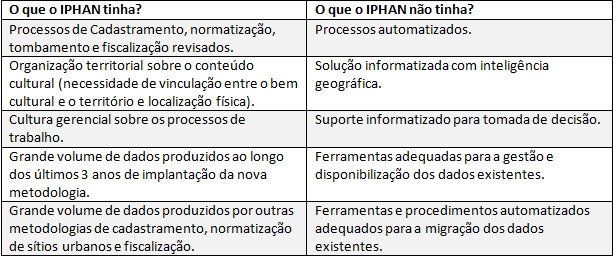
\includegraphics[scale=1.0]{figuras/problemas.png}
		\caption{Visão Geral da Situação do IPHAN}
		\label{problemas}
\end{figure}

Portanto, a solução informatizada é apontada como um caminho adequado para endereçar as dificuldades citadas, pois possibilitaria a execução de vários processos do IPHAN (cadastramento, normatização, fiscalização e planejamento) de maneira integrada, garantindo agilidade na produção da informação. 

O sistema proposto é formado por 7 módulos:

\begin{itemize}
\item Módulo 1 - Conhecimento;
\item Módulo 2 - Análise e Gestão;
\item Módulo 3 - Cadastro;
\item Módulo de Administração de Usuários;
\item Módulo de Fiscalização;
\item Módulo de Cadastro Auxiliares;
\item Módulo de Relatórios Adicionais.
\end{itemize}

\subsection[Objetivos da Contratação]{Objetivos da Contratação}

Os objetivos da contratação são:

\begin{itemize}
\item Automatizar o processo de trabalho decorrente da metodologia de inventário, cadastramento, análise e gestão do patrimônio material, denominado Sistema Integrado de Conhecimento e Gestão (SICG);
\item Centralizar as diversas bases de informações utilizadas pelo Departamento de Patrimônio Material e Fiscalização (DEPAM) em uma base de dados única, possibilitando integração futura com bases de dados de outros departamentos do IPHAN,   o problema atual de falta de integração, da dispersão e da redundância dos dados;
\item Possibilitar a descontinuidade gradativa de 100\% das bases de dados isolados, de caráter local ou descentralizado existentes no DEPAM;
\item Mapear as informações produzidas pelas diversas coordenações do DEPAM, pelas Superintendências e Escritórios Técnicos, pelos parceiros do Sistema Nacional de Patrimônio Cultural (SNPC), e as informações presentes no Arquivo Central do IPHAN, por meio de dados geográficos convergentes;
\item Possibilitar a realização de análises territoriais e de uma visão territorial das ações do DEPAM, provendo atributos de tamanho, proximidade, área, localização, topologia e outros, por meio de dados georreferenciados;
\item Consolidar informações originidas nas diversas coordenações do DEPAM, pelas Superintendências e Escritórios Técnicos, pelos parceiros do SNPC e uma base de dados geográfica de alta escalabilidade e que contenha 100\% das informações georreferenciadas;
\item Garantir celeridade no processo decisório, por meio da entrega de informações consistentes, precisos e que sejam entregues em tempo hábil, evitando ônus para a administração pública;
\item Possibilitar a redução do tempo e esforço necessário para a compilação das informações do DEPAM, advindas da recuperação e do cruzamento de produção das unidades do IPHAN de todo o pais. Espera-se que o tempo médio de resposta para compilação das informações seja reduzido de 30 dias para resposta em tempo real.
\end{itemize}

\subsection[Papéis e Responsabilidades]{Papéis e Responsabilidades}

Os papéis e responsabilidades são definidos na figura \ref{papeis} conforme a Instrução Normativa nº 04.

\begin{figure}[H]
		\centering
			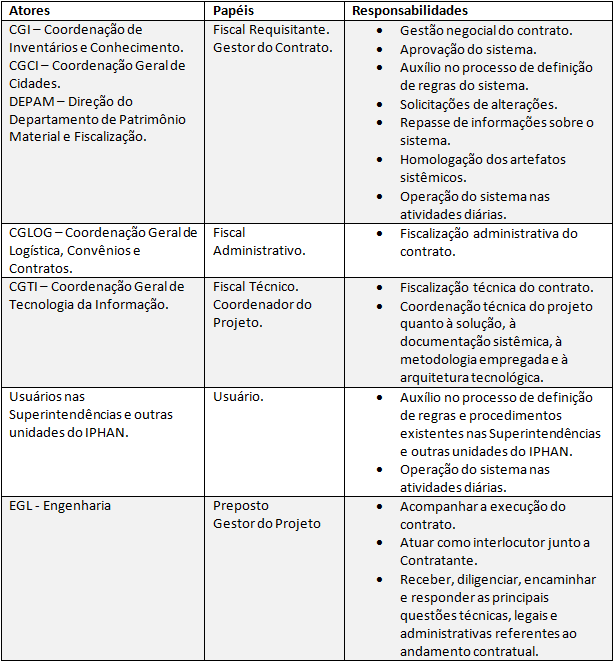
\includegraphics[scale=1.0]{figuras/papeis.png}
		\caption{Papéis e Responsabilidades do Contrato}
		\label{papeis}
\end{figure}


\subsection[Metodologia de Trabalho]{Metodologia de Trabalho}

\textbf{Forma de Encaminhamento das Ordens de Serviço}

Toda ordem de serviço será repassada pessoalmente ao preposto da contratada.


\textbf{Ciclos}

Todo o sistema será desenvolvido de forma iterativa e incremental, por meio de ciclos, ao longo de toda a vigência contratual, até sua conclusão total. O desenvolvimento e, por consequência, o repasse de conhecimento à contratada será feito por ciclos de planejamento e reuniões de levantamento de requisitos e aprendizado. Cada ciclo tem duração de 2 a 4 semanas.

O Ciclo de Planejamento (Sprint 0) tem como objetivo o planejamento de todo o projeto.

Os Ciclo de Desenvolvimento (Sprints de 1 a 24) tem como objetivo o desenvolvimento do sistema.

O Ciclo de Implantação (Penúltima Sprint) tem como objetivo a implantação do sistema.

O Ciclo de Encerramento (Última Sprint) tem como objetivo o treinamento dos seus usuários e o encerramento do projeto.

\textbf{Reuniões}

Cada ciclo teve uma Reunião de Planejamento no início do mesmo e uma Reunião de Encerramento ao final do mesmo.

Na Reunião de Planejamento, a Contratada apresentou à Contratante uma proposta de Ordem de Serviço para o ciclo em planejamento. A Contratante emitiu parecer sobre a proposta. Aprovada a proposta, a Contratante, por meio de Ordem de Serviço, autorizou a Contratada a executar o ciclo planejado.

Na Reunião de Encerramento, a Contratada entregou e apresentou à Contratante o conjunto de produtos resultantes da execução do respectivo ciclo.

Os produtos entregues pela Contratada tinha um prazo de no máximo um ciclo para serem homologados pela Contratante.

\section[Caracterização da Solução]{Caracterização da Solução}

Para desenvolver um modelo de contratação de fornecedores de \textit{software} baseado em Scrum e Kanban, o IPHAN definiu alguns procedimentos que deveriam ser feitos com o foco na minimização dos riscos da execução contratual e na obtenção do sucesso no contrato de terceirização. O \textit{framework} utilizado não é considerado o mais relevante, mas sim os valores e princípios do Manifesto Ágil, além do atendimento à legislação vigente. 

As metodologias ágeis foram utilizadas como o meio para atingir o sucesso ou para identificar de forma rápida os riscos iminentes. O sucesso contratual pode ser entendido como aquele contrato que atende às necessidades do órgão, com sistemas, sem comprometer o erário (tesouro público). Assim, para atingir sucesso em um contrato é preciso que pelos menos esses três procedimentos sejam realizados: 
\begin{itemize}
\item Definir premissas nos artefatos desde o planejamento da contratação;
\item Alinhar diretrizes e condições com a Direção de TI;
\item Convalidar com a Alta Administração, ou seja, validar e sustentar essas diretrizes durante o contrato.
\end{itemize}

A lista de práticas ágeis utilizadas no projeto SICG para a gestão do contrato estão na Tab. (6).

\begin{table}[H]
\center
\footnotesize
\begin{tabular}{|c|c|c|}
\hline
 Definição de Pronto              &   Histórias de Usuário.              \\ \hline
Planejamento das Iterações.  &  Backlog do Produto.           \\ \hline
  Backlog da Sprint.             &   Quadro Kanban.              \\ \hline
Burndown Charts.         &  Retrospectivas.            \\ \hline
Tempo de Ciclo (Lead time).         &  Revisão de Código.               \\ \hline
\end{tabular}
\caption{Práticas Ágeis adotadas pelo IPHAN}
\end{table}


Com isso, foram definidas algumas premissas que devem orientar o planejamento e execução do contrato. A saber: 
\begin{itemize}
\item O órgão não deve definir, ou exigir, o uso de Metodologia Ágil da entidade contratada. Não defina Metodologia de Desenvolvimento de Software (MDS), mas sim a
forma de gerenciar as demandas (ordens de serviço), os produtos que devem ser entregues e seus critérios de aceitação. 
\item A recontagem de Pontos por Função nos moldes do roteiro do SISP com metodologia ágil que pode mudar constantemente é um risco. É preciso alterar o percentual definido para a alteração, manutenção ou refatoração de uma funcionalidade, definir corretamente o conceito de manutenção evolutiva, refatoração e alteração de requisito e evidenciar no processo o custo de uma alteração e fazer com que o gestor negocial, que pediu a alteração, assine a ordem de serviço e ateste a nota fiscal;
\item Só abra uma Ordem de Serviço (OS) por vez e por projeto. Pode-se ter várias OS abertas com a mesma Contratada, porém, será uma OS para cada projeto e uma OS por \textit{Sprint}; Além disso, nunca comece oficialmente a próxima demanda sem receber ou finalizar a demanda anterior. Caso uma OS não estiver atendendo o que foi solicitado, ou por uma mudança negocial essa OS não for necessária, cancele-a e abra outra ordem de serviço que atenda a nova exigência do gestor contratual;
\item Não gerencie atrasos ou defeitos. No fim da \textit{Sprint}, receba o que estiver pronto, mesmo que não seja tudo que foi solicitado. Se nada foi entregue é uma ausência de entrega, não existe atraso, a \textit{Sprint} é considerada perdida. O produto não entregue ou com defeito dever voltar para fila de demandas e entrará na próxima OS ou \textit{Sprint} se o gestor negocial a quiser novamente, nunca aceite que corrijam um produto com defeito dentro da mesma OS;
\item Entenda a demanda antes de executá-la. É preciso planejar, pelo menos, com quantas ordens de serviço o projeto será validado, qual o processo de negócio que será desenvolvido, como será feita a gestão de demandas e qual será a demanda da próxima \textit{Sprint} ou OS;
\item Não aceite documentos sem sistemas. É importante ter em mente que não deve-se aceitar entregas apenas de documentação sem um produto funcional;
\item Acredite na evolução da empresa. No começo, a empresa contratada poderá não conseguir entregar o que foi solicitado ou entregar um produto funcional, no entanto, progressivamente ela irá se adequar ao processo e evoluir. 
\end{itemize} 

Com essas premissas definidas o órgão construiu um Kanban para auxiliar a Gestão de Demandas. 

O Kanban definido pelo IPHAN possui quatro colunas ou raias e está ilustrado na Fig. (\ref{kanban1}).

\begin{figure}[H]
		\centering
		
			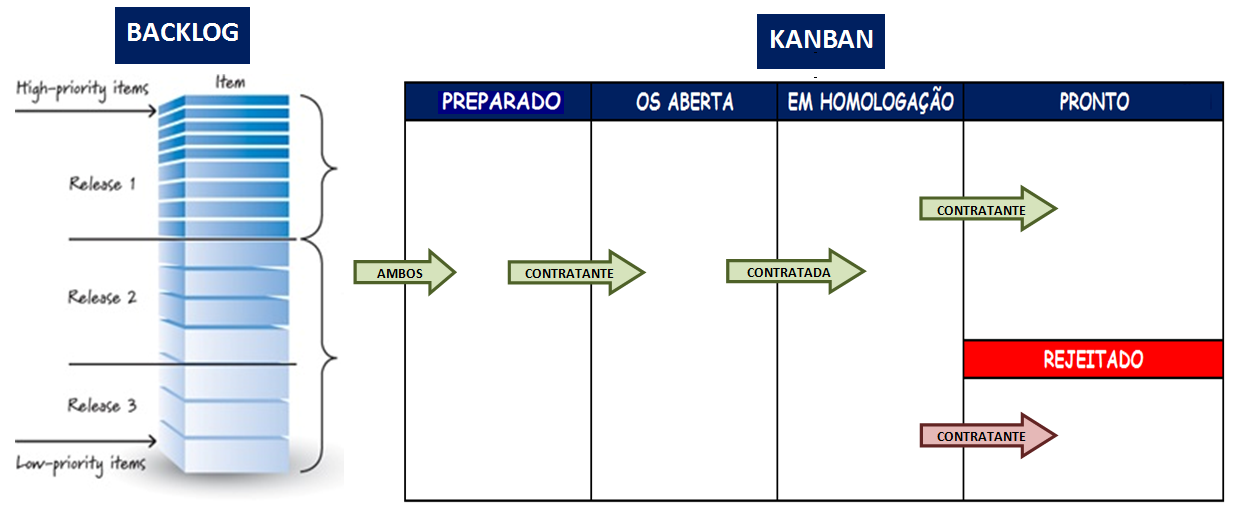
\includegraphics[scale=0.5]{figuras/kanbanIPHAN1.png}
		\caption{Quadro Kanban (imagem disponível em http://www.slideshare.net/herbertparente/contratao-de-fbrica-de-software-metodologia-gil)}
	\label{kanban1}
\end{figure}

A primeira raia do Kanban diz respeito aos itens que estão no estado “Preparado”. A condição de transição para esta raia pode ser feita da forma que o órgão quiser (\ref{kanban2}). Por exemplo, os itens com mais prioridade podem ser os primeiros a irem para esta coluna. É importante que a definição de “Preparado” e a definição de “Pronto” estejam bem claras para todos os envolvidos.  

\begin{figure}[H]
		\centering
		
			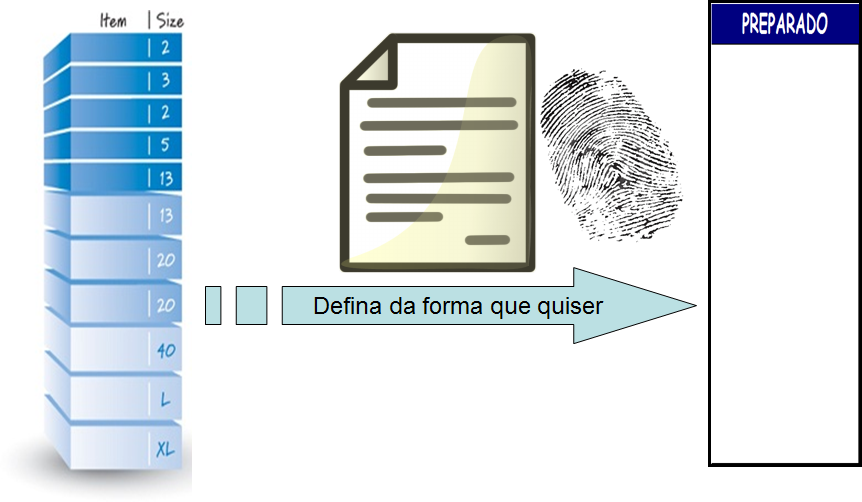
\includegraphics[scale=0.5]{figuras/kanbanIPHAN2.png}
		\caption{Transição para a raia Preparado (imagem disponível em http://www.slideshare.net/herbertparente/contratao-de-fbrica-de-software-metodologia-gil)}
		\label{kanban2}
\end{figure}

A transição de um item da raia “Preparado” para a raia “OS Aberta” ocorre na abertura de uma ordem de serviço (\ref{kanban3}). Ao observar o processo do MIDAS, percebe-se que essa transição ocorre após o planejamento da \textit{sprint}, no subprocesso \textit{Sprint}, onde uma ordem de serviço de desenvolvimento é aberta  com os itens que devem ser desenvolvidos para aquela \textit{sprint} e o desenvolvimento é iniciado. 

\begin{figure}[H]
		\centering
		
			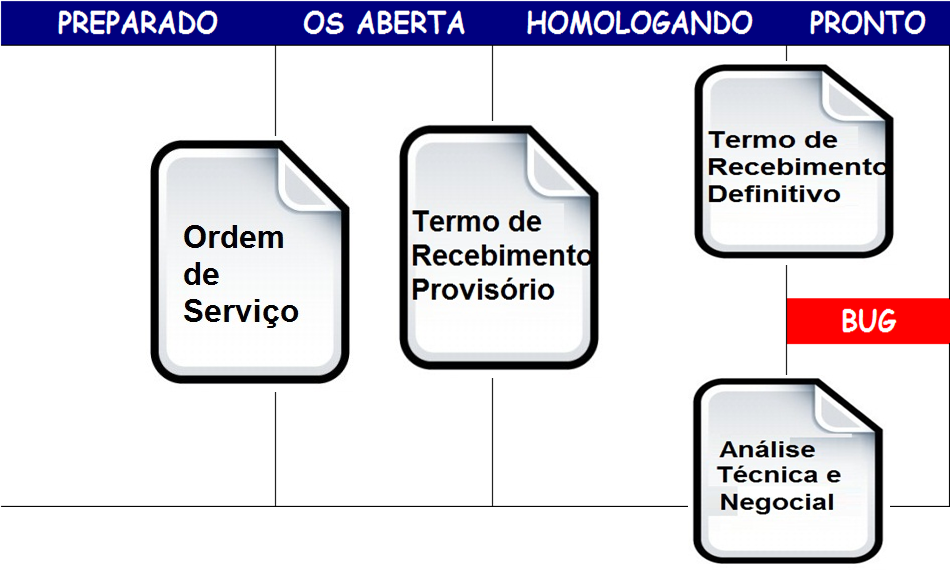
\includegraphics[scale=0.5]{figuras/kanbanIPHAN3.png}
		\caption{Transição entre raias (imagem disponível em http://www.slideshare.net/herbertparente/contratao-de-fbrica-de-software-metodologia-gil)}
		\label{kanban3}
\end{figure}

A transição da raia “OS Aberta” para a raia “Homologando” ocorre quando o Termo de Recebimento Provisório é emitido (Fig. 14). Ao se observar o subprocesso de Realizar Ateste Técnico, percebe-se que essa transição ocorre na atividade “Receber Produtos”. Esta tem como entrada a ordem de serviço da fase e como saída o termo de recebimento provisório. Com a emissão do termo de recebimento provisório, os produtos recebidos entram na processo de homologação. 

A transição da raia “Homologando” para a raia “Pronto” ocorre quando o Termo de Recebimento Definitivo é emitido, ou seja, quando todos os produtos que foram anteriormente entregues são verificados e aprovados (\ref{kanban3}). Para tanto são aferidos a aderência aos padrões técnicos e aos requisitos a partir de uma análise técnica e negocial, realizadas conjuntamente pelo Fiscal do Contrato e o Gestor de Negócio. Se forem detectados defeitos nos produtos entregues ou se eles forem rejeitados ou tiverem necessidade de refatoração, eles retornam para a fila de demandas, iniciando novamente o ciclo. A sinalização de rejeitado ou \textit{bug} diz respeito a funcionalidade que foi rejeitada por não atender o que foi pedido tanto funcionalmente quanto tecnicamente. A sinalização de refatoração diz respeito a mudança que é pedida em uma funcionalidade depois de ela já ter sido implementada. Para que uma funcionalidade entre nessa sinalização é preciso que o gestor de negócio assuma a responsabilidade pelos impactos que a mudança causará no custo, tempo e escopo.

Vale ressaltar que é importante que o trabalho em progresso (WIP) seja limitado conforme o que é conceituado no método Kanban. O IPHAN definiu um limite de 200 Pontos por Função por ciclo de trabalho (\ref{kanban4}). 

\begin{figure}[h]
		\centering
		
			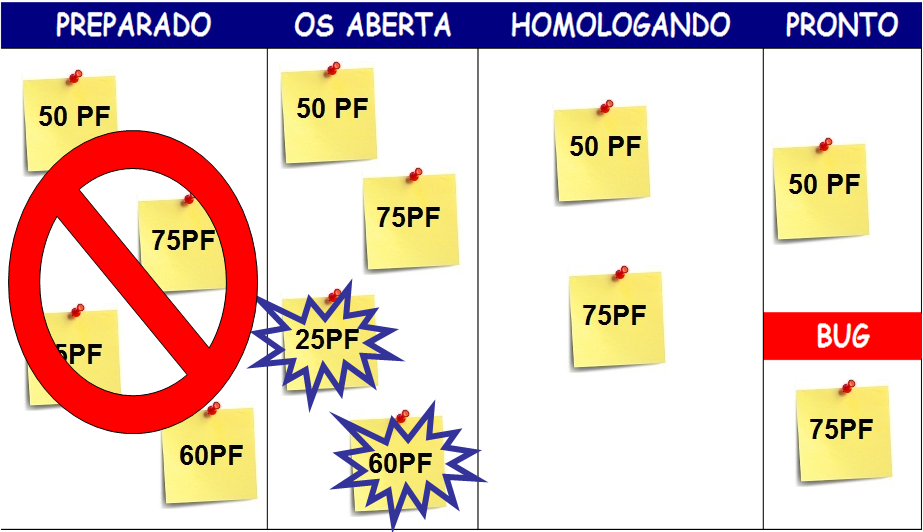
\includegraphics[scale=0.5]{figuras/kanbanIPHAN4.png}
		\caption{Limitação de WIP (imagem disponível em http://www.slideshare.net/herbertparente/contratao-de-fbrica-de-software-metodologia-gil)}
		\label{kanban4}
\end{figure}

É importante sempre valorizar a entrega de produto funcional e não pagar por apenas documentação. Assim, o IPHAN dividiu a forma de pagamento da contratada em percentuais, de acordo com a fase, valorizando a fase de execução, como ilustrado na Tab. (7). Na Sprint 18 do projeto SICG, ocorreu uma mudança acordada com a empresa contratada de modificar o pagamento da fase de execução para 100\%, pois o fluxo de caixa da empresa estava curto. Valorizando - se ainda mais a fase de execução.


\begin{table}[H]
\center
\footnotesize
\begin{tabular}{|p{6cm}|p{6cm}|}
  \hline
   \textbf{Fase} & \textbf{Percentual de Pagamento}\\
    \hline
   Planejamento (1 vez) & 5\%\\
   \hline    
   Execução (n vezes) & 75\%\\
    \hline
   Implantação (1 vez) & 10\%\\
   \hline
   Encerramento (1 vez) & 10\%\\
   \hline
\end{tabular}
\caption{Modelo de Remuneração do projeto SICG}
\end{table}


Outra técnica importante que foi construída diz respeito a parelização das atividades \ref{kanban5}. Enquanto uma ordem de serviço está na etapa de homologação, outra ordem de serviço pode ser preparada, evitando que o fluxo do processo pare e haja desperdício. 

\begin{figure}[H]
		\centering
		
			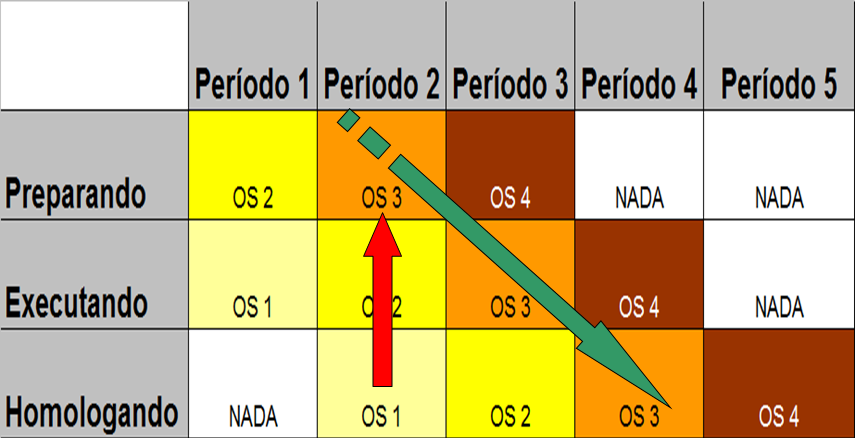
\includegraphics[scale=0.5]{figuras/kanbanIPHAN5.png}
		\caption{Parelização de Atividades (imagem disponível em http://www.slideshare.net/herbertparente/contratao-de-fbrica-de-software-metodologia-gil)}
		\label{kanban5}
\end{figure}

O Kanban evidencia a aderência de utilização de métodos ágeis. A paralelização das atividades, que evita desperdícios de trabalho, evidencia a aderência ao Lean no Desenvolvimento de \textit{Software}. Assim, conclui-se que as premissas utilizadas como base para o desenvolvimento do Kanban foram baseadas tanto nos princípios ágeis quanto nos princípios do Lean. Após alguns meses de aplicação dessa solução o órgão deu início a construção da Metodologia IPHAN de Gestão de Demandas de Desenvolvimento Ágil de \textit{Software} (MIDAS). Uma parte do MIDAS pode ser visualizada no Anexo B. 


\section[Análise dos Dados]{Análise dos Dados}

Nesta seção serão apresentados os resultados dos dados coletados categorizados em três efeitos: entrega de ordens de serviço, satisfação do cliente e qualidade interna do código fonte. As subseções a seguir têm o objetivo de responder diretamente às questões específicas de pesquisa definidas no Capítulo 5.

\subsection[Efeitos sobre a entrega de ordens de serviço]{Efeitos sobre a entrega de ordens de serviço}

A partir dos dados coletados da documentação dos Processos do projeto SICG foram calculadas as métricas para responder as questões de pesquisa QE1. A QE9. que caracterizam os efeitos sobre a entrega de ordens de serviço do uso de métodos ágeis na gestão do contrato de fornecedores de desenvolvimento de software.

A Figura \ref{resultadosmetricas} apresenta os resultados das métricas para cada uma das questões de pesquisa anteriormente mencionadas.

\begin{figure}[H]
		\centering
			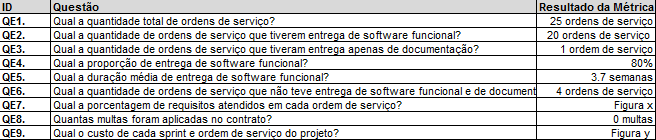
\includegraphics[scale=1.0]{figuras/resultadosmetricas.png}
		\caption{Resultados Métrica de QE1. a QE9.}
		\label{resultadosmetricas}
\end{figure}

A Figura \ref{porcentagemrequisitos} apresenta a porcentagem de requisitos atendidos em cada ordem de serviço ou sprint, respondendo assim a questão de pesquisa QE7.

\begin{figure}[H]
		\centering
			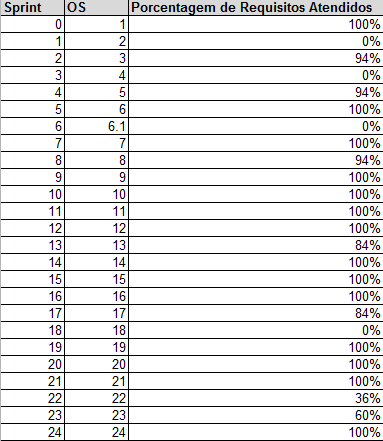
\includegraphics[scale=1.0]{figuras/porcentagemrequisitos.png}
		\caption{Porcentagem de Requisitos Atendidos por Ordem de Serviço}
		\label{porcentagemrequisitos}
\end{figure}

 A média geral de requisitos atendidos ao longo do projeto de acordo com os dados levantados da documentação foi de 78\%, o que coincide com a percepção dos envolvidos no projeto: 75\% dos envolvidos responderam ao questionário que a percepção geral de requisitos atendidos durante o projeto estava entre 70\% e 90\%.

A Figura \ref{custo} apresenta o custo de cada ordem de serviço ou sprint, respondendo assim a questão de pesquisa QE9. Como pode ser observado, nas ordens de serviço que tiverem a porcentagem de requisitos atendidos como 0\% não houve remuneração para a contratada. O custo estimado do contrato antes da contratação era de R\$ 990,000. Portanto, o custo final foi próximo do custo estimado, ultrapassando apenas 1,8\%.

\begin{figure}[H]
		\centering
			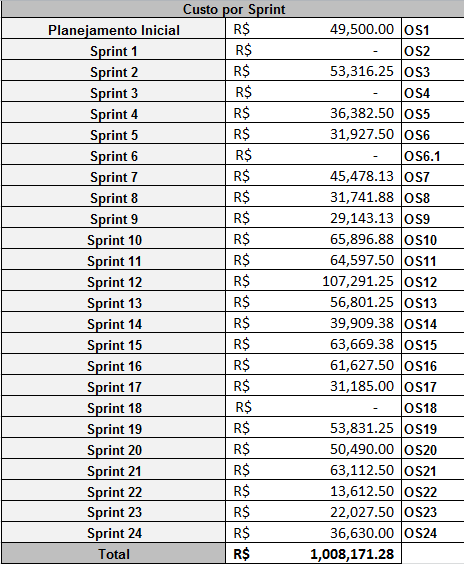
\includegraphics[scale=1.0]{figuras/custo.png}
		\caption{Custo por Ordem de Serviço}
		\label{custo}
\end{figure}

É importante destacar que apesar das sprints 1, 3, 6 e 18 não tiverem sido faturadas, não houve aplicação de multa para a contratada. Pois, conforme a solução caracterizada anteriormente, o órgão optou por modificar o modelo de remuneração e considera o aprendizado e a adaptação da empresa ao tipo de metodologia de gestão de contrato que está sendo aplicado. Além disso, o fato de a empresa não ter um pagamento em seu fluxo de caixa já é penalização suficiente para que a empresa faça a adequação do seu processo de trabalho.

\subsection[Efeitos sobre a satisfação do cliente]{Efeitos sobre a satisfação do cliente}

O cliente do projeto SICG é representado pelo papel de dono do produto, que também atuou como gestor do contrato, e por todos os envolvidos no projeto por parte do IPHAN. Os IPHAN nunca havia participado anteriormente de um projeto onde a gestão do contrato era realizada com o uso de métodos ágeis, portanto, a experiência dos envolvidos no projeto com métodos ágeis era pouca. Para coletar a opinião do cliente acerca das questões de pesquisa QE10  e QE11 foi aplicado um questionário.

A Figura \ref{visibilidade} apresenta a visibilidade do processo de todos os envolvidos no projeto por parte do IPHAN. Cerca de 80\% dos envolvidos no projeto considerou a visibilidade do processo como "Alta", dentre eles o gestor do contrato.

\begin{figure}[H]
		\centering
			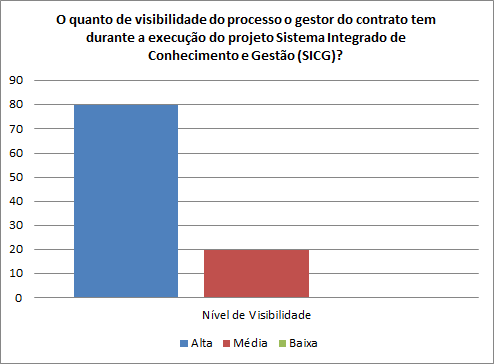
\includegraphics[scale=1.0]{figuras/visibilidade.png}
		\caption{Nível de Visibilidade do Processo do Projeto SICG}
		\label{visibilidade}
\end{figure}

A Figura \ref{satisfacao} apresenta o resultado de satisfação do IPHAN com relação ao produto entregue. De forma unânime foi considerado como "Satisfeito" o produto entregue pela empresa contratada. 

\begin{figure}[H]
		\centering
			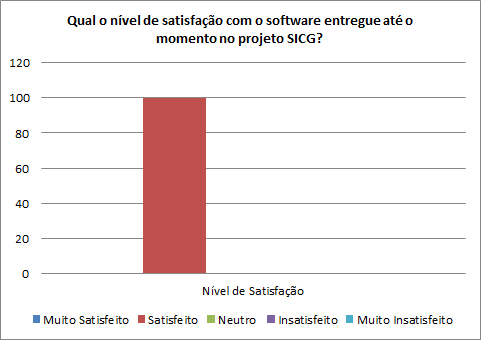
\includegraphics[scale=1.0]{figuras/satisfacao.png}
		\caption{Nível de Satisfação do Produto Entregue do Projeto SICG}
		\label{satisfacao}
\end{figure}

\subsection[Efeitos sobre a qualidade do código]{Efeitos sobre a qualidade do código}

A qualidade do código fonte do SICG pode ser avaliada por meio de métricas. Neste trabalho foram selecionadas as métricas de código fonte levantadas e categorizadas por MEIRELLES: métricas de tamanho e complexidade e métricas de orientação à objetos. 

As métricas de tamanho e complexidade selecionadas são: 

\textbf{LOC (Lines of Code):} número de Linhas de Código foi uma das primeiras métricas
utilizadas para medir o tamanho de um software. São contadas apenas as linhas
executáveis, ou seja, são excluídas linhas em branco e comentários \cite{Jones91}.

 \vspace{\onelineskip} 

\textbf{ACCM (Average Cyclomatic Complexity per Method):} média da Complexidade
Ciclomática por Método mede a complexidade dos métodos ou funções
de um programa. Essa métrica pode ser representada através de um grafo de fluxo
de controle \cite{McCabe76}. O uso de estruturas de controle, tais como, if, else,
while aumentam a complexidade ciclomática de um método.

 \vspace{\onelineskip}

\textbf{AMLOC (Average Method Lines of Code)} - essa medida indica se o código está bem distribuído entre os métodos. Quanto maior, mais pesados são os métodos. É preferível ter muitas operações pequenas e de fácil entendimento que poucas operações grandes e complexas \cite{Meirelles2013}.



 \vspace{\onelineskip} 

As métricas de orientação à objetos selecionadas são:

\textbf{ACC (Afferent Connections per Class):} conexões Aferentes por Classe é o número
total de classes externas de um pacote que dependem de classes de dentro desse
pacote. Quando calculada no nível da classe, essa medida também é conhecida como
Fan-in da classe, medindo o número de classes das quais a classe é derivada e, assim,
valores elevados indicam uso excessivo de herança múltipla \cite{McCabe94} \cite{Chidamber94}.

 \vspace{\onelineskip} 

 \textbf{ANPM (Average Number of Parameters per Method)} - calcula a média de parâmetros dos métodos da classe. Seu valor mínimo é zero e não existe um limite máximo para o seu resultado, mas um número alto de parâmetros pode indicar que um método pode ter mais uma responsabilidade \cite{Basili1987}


 \vspace{\onelineskip} 

\textbf{CBO (Coupling Between Objects)} -  é o número total de classes dentro de um pacote que dependem de classes externas ao pacote. Quando calculada no nível da classe, essa medida também é conhecida como Fan-out da classe \cite{Chidamber94}

 \vspace{\onelineskip} 

\textbf{DIT (Depth of Inheritance Tree):} profundidade da Árvore de Herança é o número
de superclasses ou classes ancestrais da classe sendo analisada. São contabilizadas
apenas as superclasses do sistema, ou seja, as classes de bibliotecas não são
contabilizadas. Nos casos onde herança múltipla é permitida, considera-se o maior
caminho da classe até uma das raízes da hierarquia. Quanto maior for o valor DIT,
maior é o número de atributos e métodos herdados, e, portanto,maior é a complexidade
\cite{Shih97}.

 \vspace{\onelineskip} 

\textbf{LCOM4 (Lack of Cohesion in Methods):} falta de Coesão entre Métodos. Originalmente
proposto por \citeonline{Chidamber94} como LCOM não teve uma
grande aceitabilidade. Após críticas e sugestões a métrica foi revisada por \citeonline{LCOM4}, que propôs a LCOM4. Para calcular LCOM4 de um módulo, é
necessário construir um gráfico não-orientado em que os nós são os métodos e atributos
de uma classe. Para cada método, deve haver uma aresta entre ele e um outro
método ou variável que ele usa. O valor da LCOM4 é o número de componentes
fracamente conectados nesse gráfico.


 \vspace{\onelineskip} 

\textbf{NOC (Number of Children):} número de Filhos é o número de subclasses ou classes
filhas que herdam da classe analisada \cite{Rosenberg97}. Deve se ter
cautela ao modificar classes com muitos filhos, pois uma simples modificação de
assinatura de um método, pode criar uma mudança em muitas classes.


 \vspace{\onelineskip} 

\textbf{NOM (Number of Methods):} número de Métodos é usado para medir o tamanho
das classes em termos das suas operações implementadas. Essa métrica é usada para
ajudar a identificar o potencial de reúso de uma classe. Em geral, as classes com
um grande número de métodos são mais difíceis de serem reutilizadas, pois elas são
propensas a serem menos coesas \cite{Lorenz94}.


 \vspace{\onelineskip} 

\textbf{NPA (Number of Public Attributes)} - mede o encapsulamento. Os atributos de uma classe devem servir apenas às funcionalidades da própria classe. Portanto, boas práticas de programação recomendam que os atributos de uma classe devem ser manipulados através dos métodos de acesso \cite{beck1997smalltalk}



 \vspace{\onelineskip} 

\textbf{RFC (Response For a Class):} respostas para uma Classe é número de métodos
dentre todos os métodos que podem ser invocados em resposta a uma mensagem
enviada por um objeto de uma classe \cite{Sharble93}.



 \vspace{\onelineskip} 

Um dos objetivos científicos do estudo de \citeonline{Meirelles2013} foi a identificação das distribuições estatísticas do valores das métricas apresentadas anteriormente em 38 projetos
de software livre. A partir de cada uma das distribuições estatísticas \citeonline{Meirelles2013} classificou as métricas de código fonte de acordo com a frequência dos valores apresentados,
com os intervalos: muito frequente, frequente, pouco frequente e não frequente. Para simplificar o entendimento das métricas de código fonte, Morais interpretou os rótulos dos
intervalos de frequência definidos por \citeonline{Meirelles2013} em em rótulos qualitativos, tal como a Tab. (8). 

\begin{table}[!ht]
	\begin{center}
	 \begin{tabular}{|l|l|}
		\hline
		\textbf{Intervalo de Frequência} & \textbf{Rótulo Qualitativos} \\ \hline
		Muito Frequente & Excelente \\ \hline
		Frequente       & Bom       \\ \hline
		Pouco Frequente & Regular   \\ \hline
		Não Frequente   & Ruim      \\ \hline
		\end{tabular}
		\caption{Nome dos Intervalos de Frequência e Qualitativos}
		\label{nomes}
		\end{center}
		\end{table}


Posteriormente, apresenta-se a Tabela 3, retirada do
estudo de \citeonline{Meirelles2013}, com os intervalos encontrados para C++ e Java. Com isso, os intervalos apresentados na Tab. (9) foram os utilizados como os indicadores
de qualidade de código fonte na análise deste estudo de caso. É importante ressaltar que quando apresentarmos o resultado da análise sobre o código fonte desse estudo de caso e dissermos que o código fonte tem um rótulo "excelente" ou "ruim" para determinada métrica siginifica que esse código fonte é "excelente" ou "ruim" em comparação ao melhor projeto de software livre selecionado por \citeonline{Meirelles2013} na Linguagem Java, que foi o Open JDK8.

 \vspace{\onelineskip} 
 \vspace{\onelineskip} 
 \vspace{\onelineskip} 
 \vspace{\onelineskip} 
 \vspace{\onelineskip} 

	
\begin{longtable}{|l|l|l|}
		\hline
		
		\textbf{Métrica} & \textbf{Rótulos Qualitativos} &  \textbf{Intervalos Qualitativos}  \\ \hline
		 % Métrica de Tamanho e Complexidade


		 %------------------------------- Tomcat
		 \multirow{4}{*}{LOC} 
		 & Excelente & [de 0 a 33]  \\
		 & Bom & [de 34 a 87]] \\
		 & Regular & [de 88 a 200]  \\
		 & Ruim & [acima de 200] \\ \hline
		 %---------------------------------

		 %-------------------------------  Tomcat	
		 \multirow{4}{*}{ACCM} 
		 & Excelente & [de 0 a 2,8]  \\
		 & Bom & [de 2,9 a 4,4]  \\
		 & Regular & [de 4,5 a 6,0]  \\
		 & Ruim & [acima de 6]  \\ \hline
		 %---------------------------------


		 %--------------------------------- Tomcat
		 \multirow{4}{*}{AMLOC} 
		 & Excelente & [de 0 a 8,3]  \\
		 & Bom & [de 8,4 a 18]  \\
		 & Regular & [de 19 a 34]  \\
		 & Ruim & [acima de 34]  \\ \hline
		 %---------------------------------

		 % Métricas de Orientação à Objetos

		 %------------------------------- Tomcat
		 \multirow{4}{*}{ACC} 
		 & Excelente & [de 0 a 1] \\
		 & Bom & [de 1,1 a 5]  \\
		 & Regular & [de 5,1 a 12] \\
		 & Ruim & [acima de 12] ] \\ \hline
		 %---------------------------------


		 %--------------------------------- Tomcat
		 \multirow{4}{*}{ANPM} 
		 & Excelente & [de 0 a 1,5] \\
		 & Bom & [de 1,6 a 2,3] ] \\
		 & Regular & [de 2,4 a 3,0]  \\
		 & Ruim & [acima de 3] \\ \hline
		 %---------------------------------

		 %--------------------------------- Tomcat
		 \multirow{4}{*}{CBO} 
		 & Excelente & [de 0 a 3]  \\
		 & Bom & [de 4 a 6] ] \\
		 & Regular & [de 7 a 9]  \\
		 & Ruim & [acima de 9] \\ \hline
		 %---------------------------------

		 %------------------------------- Tomcat
		 \multirow{4}{*}{DIT} 
		 & Excelente & [de 0 a 2]   \\
		 & Bom & [de 3 a 4]  ] \\
		 & Regular & [de 5 a 6]   \\
		 & Ruim & [acima de 6]  \\ \hline
		 %---------------------------------

		 %------------------------------- Tomcat
		 \multirow{4}{*}{LCOM4} 
		 & Excelente & [de 0 a 3]  \\
		 & Bom & [de 4 a 7]  \\
		 & Regular & [de 8 a 12]   \\
		 & Ruim & [acima de 12]  ] \\ \hline
		 %---------------------------------



		 %------------------------------- Tomcat
		 \multirow{4}{*}{NOC} 
		 & Excelente & [0]  \\
		 & Bom & [1 a 2]   \\
		 & Regular & [3]  ] \\
		 & Ruim & [acima de 3]   \\ \hline
		 %---------------------------------



		 %------------------------------- Tomcat 
		 \multirow{4}{*}{NOM} 
		 & Excelente & [de 0 a 8]   \\
		 & Bom & [de 9 a 17]   \\
		 & Regular & [de 18 a 27]  \\
		 & Ruim & [acima de 27]   \\ \hline
		 %---------------------------------




		 %--------------------------------- Tomcat
		 \multirow{4}{*}{NPA} 
		 & Excelente & [0]   \\
		 & Bom & [1]   \\
		 & Regular & [de 2 a 3]   \\
		 & Ruim & [acima de 3]  \\ \hline
		 %---------------------------------


		 %------------------------------- Tomcat 
		 \multirow{4}{*}{RFC} 
		 & Excelente & [de 0 a 9]   \\
		 & Bom & [de 10 a 26]  ] \\
		 & Regular & [de 27 a 59]   \\
		 & Ruim & [acima de 59]   \\ \hline
		 %---------------------------------
 	

			\caption{Intervalos de Qualidade Java}
	\end{longtable}

De forma geral, o processo realizado para a análise do código fonte do SICG foi retirado do trabalho desenvolvido por \citeonline{baufaker}, que  consiste em: executar a ferramenta Analizo sobre o código fonte do projeto SICG, o qual resultará em um arquivo .csv com os resultados númericos das métricas selecionadas, transformar o arquivo .csv em json e inserir esse arquivo na arquitetura desenvolvida por \citeonline{baufaker} na ferramenta Pentaho. Ao final desse processo, temos como resultado os gráficos para análise. 

A fim de responder a questão de pesquisa QE12 serão mostrados a seguir os resultados do processamento do código fonte do projeto SICG no que diz respeito a qualidade do código ao longo das sprints do projeto de acordo com as oito métricas selecionadas. Os rótulos de intervalos de qualidade mostrados são resultantes dos valores médios de cada métrica para todas as classes do projeto. 

As Figuras \ref{metricasprint}, \ref{metricasprint2} e \ref{metricasprint2} mostram os valores de todas as métricas ao longo das sprints do projeto.
\begin{figure}[H]
		\centering
			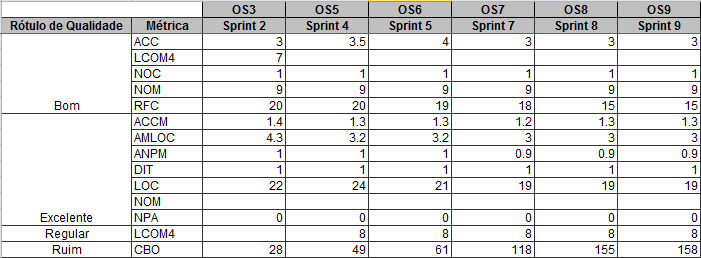
\includegraphics[scale=0.9]{figuras/metricas29.png}
		\caption{Valores das Métricas do Projeto SICG da Sprint 2 a Sprint 9}
		\label{metricasprint}
\end{figure}

\begin{figure}[H]
		\centering
			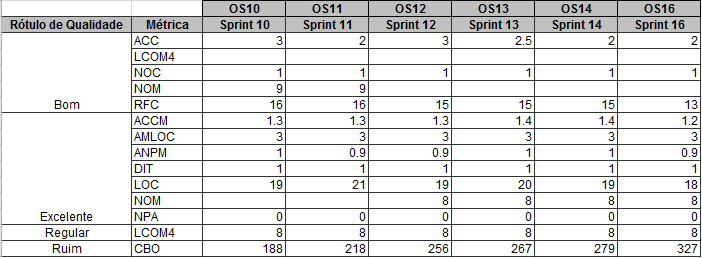
\includegraphics[scale=0.9]{figuras/metricas1016.png}
		\caption{Valores das Métricas do Projeto SICG da Sprint 10 a Sprint 16}
		\label{metricasprint2}
\end{figure}

\begin{figure}[H]
		\centering
			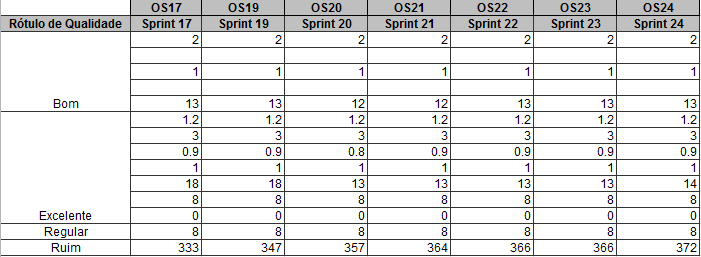
\includegraphics[scale=0.9]{figuras/metricas1724.png}
		\caption{Valores das Métricas do Projeto SICG da Sprint 17 a Sprint 24}
		\label{metricasprint3}
\end{figure}

A seguir, serão apresentados os gráficos, primeiramente, dos resultados de cada métrica de forma individual ao longo das sprints do projeto e, posteriormente, o resultado geral da qualidade do código ao longo das sprints do projeto.

\textbf{LOC (Lines of Code)}

A Figura \ref{loc} mostra a qualidade da métrica LOC. Esta métrica permanece com o intervalo de qualidade "Excelente" constante ao longo das sprints do projeto.

\begin{figure}[H]
		\centering
			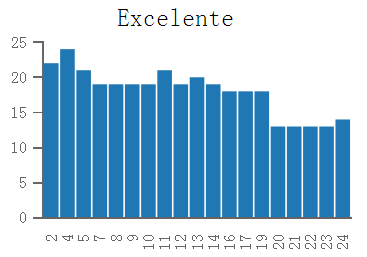
\includegraphics[scale=1.0]{figuras/loc.png}
		\caption{Qualidade da Métrica LOC nas Sprints do Projeto SICG}
		\label{loc}
\end{figure}

\textbf{ACCM (Average Cyclomatic Complexity per Method)}

A Figura \ref{accm} mostra a qualidade da métrica ACCM. Esta métrica permanece com o intervalo de qualidade "Excelente" constante ao longo das sprints do projeto.

\begin{figure}[H]
		\centering
			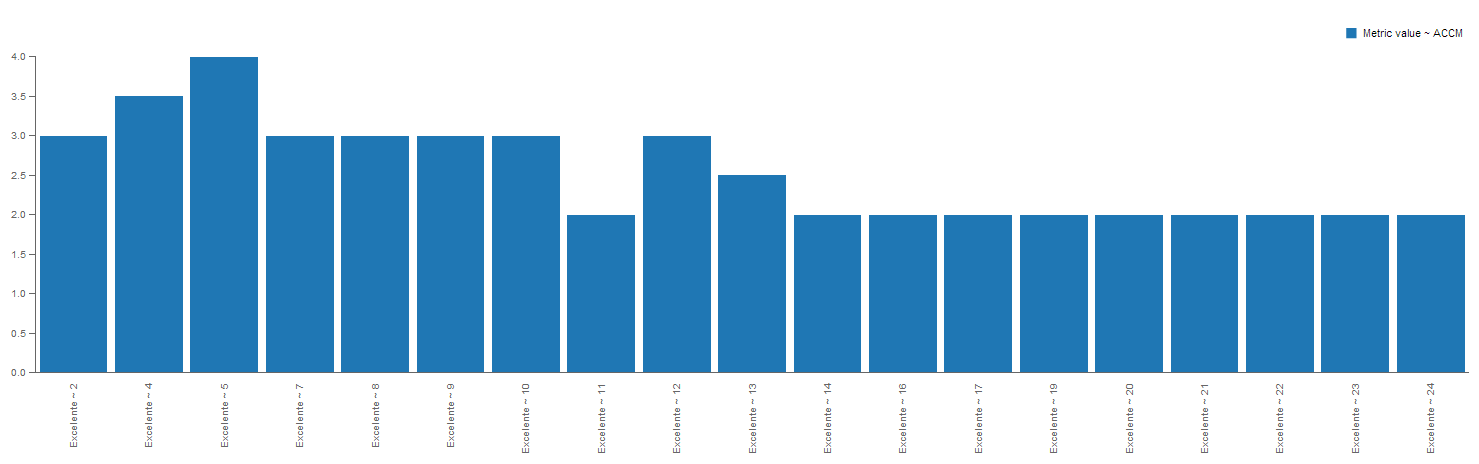
\includegraphics[scale=1.0]{figuras/accm.png}
		\caption{Qualidade da Métrica ACCM nas Sprints do Projeto SICG}
		\label{accm}
\end{figure}

\textbf{AMLOC (Average Method Lines of Code)}

A Figura \ref{amloc} mostra a qualidade da métrica AMLOC. Esta métrica permanece com o intervalo de qualidade "Excelente" constante ao longo das sprints do projeto.

\begin{figure}[H]
		\centering
			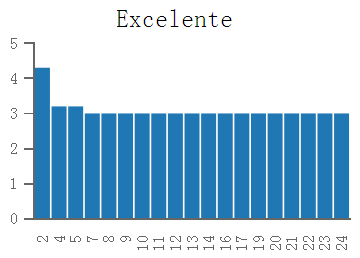
\includegraphics[scale=1.0]{figuras/amloc.png}
		\caption{Qualidade da Métrica AMLOC nas Sprints do Projeto SICG}
		\label{amloc}
\end{figure}

\textbf{ACC (Afferent Connections per Class)}

A Figura \ref{acc} mostra a qualidade da métrica ACC. Esta métrica permanece com o intervalo de qualidade "Bom" constante ao longo das sprints do projeto.

\begin{figure}[H]
		\centering
			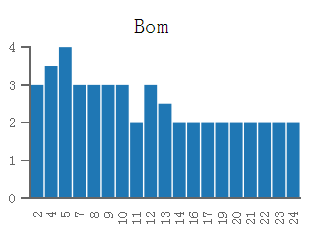
\includegraphics[scale=1.0]{figuras/acc.png}
		\caption{Qualidade da Métrica ACC nas Sprints do Projeto SICG}
		\label{acc}
\end{figure}

\textbf{ANPM (Average Number of Parameters per Method)}

A Figura \ref{anpm} mostra a qualidade da métrica ANPM. Esta métrica permanece com o intervalo de qualidade "Excelente" constante ao longo das sprints do projeto.

\begin{figure}[H]
		\centering
			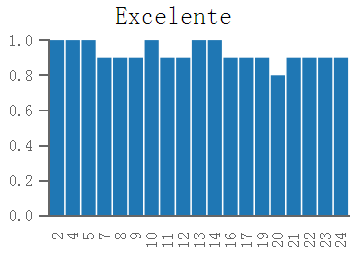
\includegraphics[scale=1.0]{figuras/anpm.png}
		\caption{Qualidade da Métrica ANPM nas Sprints do Projeto SICG}
		\label{anpm}
\end{figure}

\textbf{CBO (Coupling Between Objects)}

A Figura \ref{cbo} mostra a qualidade da métrica CBO. Esta métrica permanece com o intervalo de qualidade "Ruim" constante ao longo das sprints do projeto.

\begin{figure}[H]
		\centering
			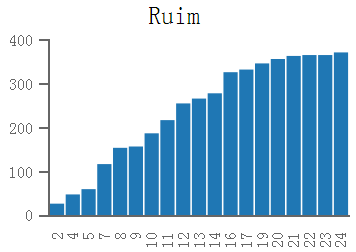
\includegraphics[scale=1.0]{figuras/cbo.png}
		\caption{Qualidade da Métrica CBO nas Sprints do Projeto SICG}
		\label{cbo}
\end{figure}

\textbf{DIT(Depth of Inheritance Tree)}

A Figura \ref{dit} mostra a qualidade da métrica DIT. Esta métrica permanece com o intervalo de qualidade "Excelente" constante ao longo das sprints do projeto.

\begin{figure}[H]
		\centering
			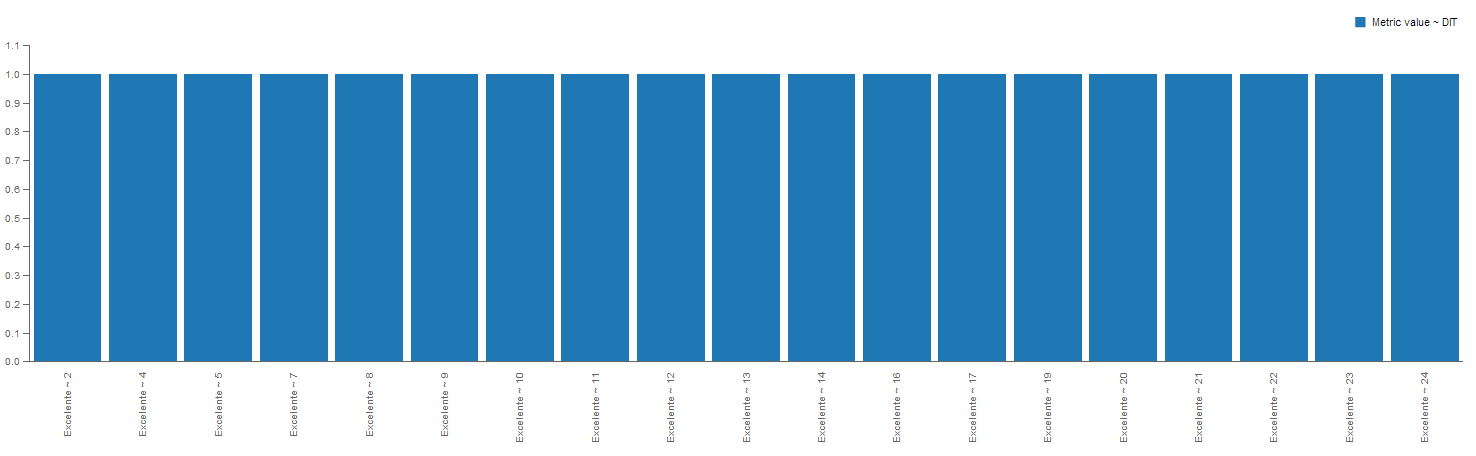
\includegraphics[scale=1.0]{figuras/dit.png}
		\caption{Qualidade da Métrica DIT nas Sprints do Projeto SICG}
		\label{dit}
\end{figure}


\textbf{LCOM4 (Lack of Cohesion in Methods)} 

A Figura \ref{lcom4} mostra a qualidade da métrica LCOM4. Esta métrica inicia com o intervalo de qualidade "Bom" na primeira sprint com entrega de software (Sprint 2) e, posteriormente, permanece com o intervalo de qualidade "Regular" constante ao longo das demais sprints do projeto.

\begin{figure}[H]
		\centering
			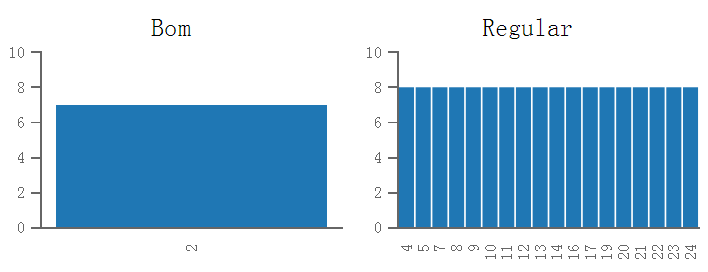
\includegraphics[scale=0.9]{figuras/lcom4.png}
		\caption{Qualidade da Métrica LCOM4  nas Sprints do Projeto SICG}
		\label{lcom4}
\end{figure}

\textbf{NOC (Number of Children)}

A Figura \ref{noc} mostra a qualidade da métrica NOC. Esta métrica permanece com o intervalo de qualidade "Bom" constante ao longo das sprints do projeto.

\begin{figure}[H]
		\centering
			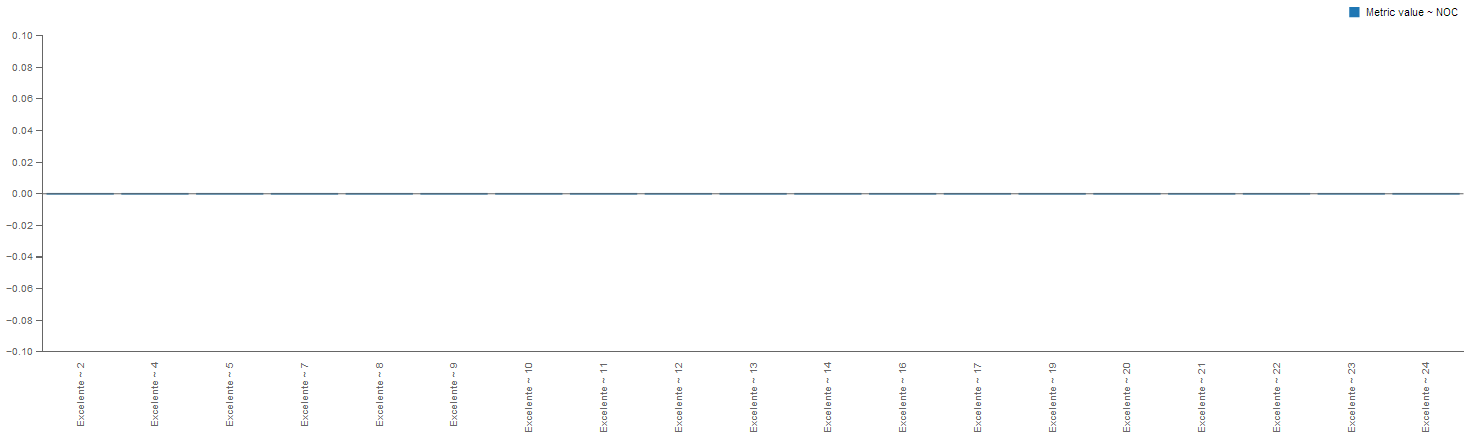
\includegraphics[scale=1.0]{figuras/noc.png}
		\caption{Qualidade da Métrica NOC nas Sprints do Projeto SICG}
		\label{noc}
\end{figure}


\textbf{NOM (Number of Methods)} 

A Figura \ref{nom} mostra a qualidade da métrica NOM. Esta métrica permanece com o intervalo de qualidade "Bom" até a Sprint 11 do projeto, a partir da Sprint 12 o código fonte obtém uma melhoria e a métrica NOM passa a ter o intervalo de qualidade "Excelente" até a última sprint analisada do projeto.

\begin{figure}[H]
		\centering
			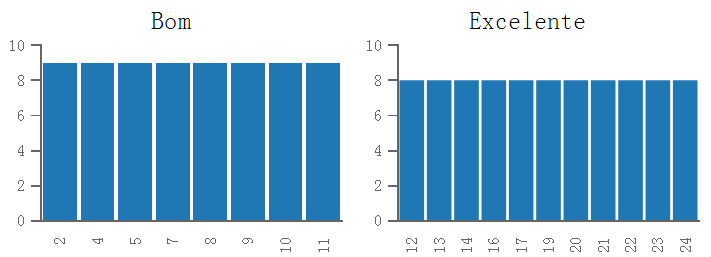
\includegraphics[scale=0.9]{figuras/nom.png}
		\caption{Qualidade da Métrica NOM nas Sprints do Projeto SICG}
		\label{nom}
\end{figure}

\textbf{NPA (Number of Public Attributes)} 

A Figura \ref{npa} mostra a qualidade da métrica NPA. Esta métrica permanece com o intervalo de qualidade "Excelente" constante ao longo das sprints do projeto.

\begin{figure}[H]
		\centering
			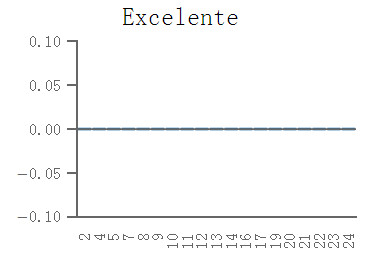
\includegraphics[scale=1.0]{figuras/npa.png}
		\caption{Qualidade da Métrica NPA nas Sprints do Projeto SICG}
		\label{npa}
\end{figure}

\textbf{RFC (Response For a Class)} 

A Figura \ref{rfc} mostra a qualidade da métrica RFC. Esta métrica permanece com o intervalo de qualidade "Bom" constante ao longo das sprints do projeto.

\begin{figure}[H]
		\centering
			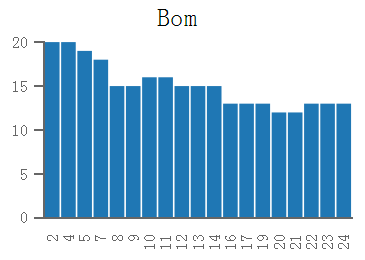
\includegraphics[scale=1.0]{figuras/rfc.png}
		\caption{Qualidade da Métrica RFC nas Sprints do Projeto SICG}
		\label{rfc}
\end{figure}

A Figura \ref{qualidadesprint} mostra a qualidade de todas as métricas analisadas ao longo das sprints do projeto desconsiderando a métrica CBO. Considerando que a Sprint 24 é a última sprint do projeto e, portanto, seria o código final, observamos uma predominância do intervalo de qualidade "Excelente", seguido do intervalo "Bom" e "Regular", respectivamente. 

\begin{figure}[H]
		\centering
			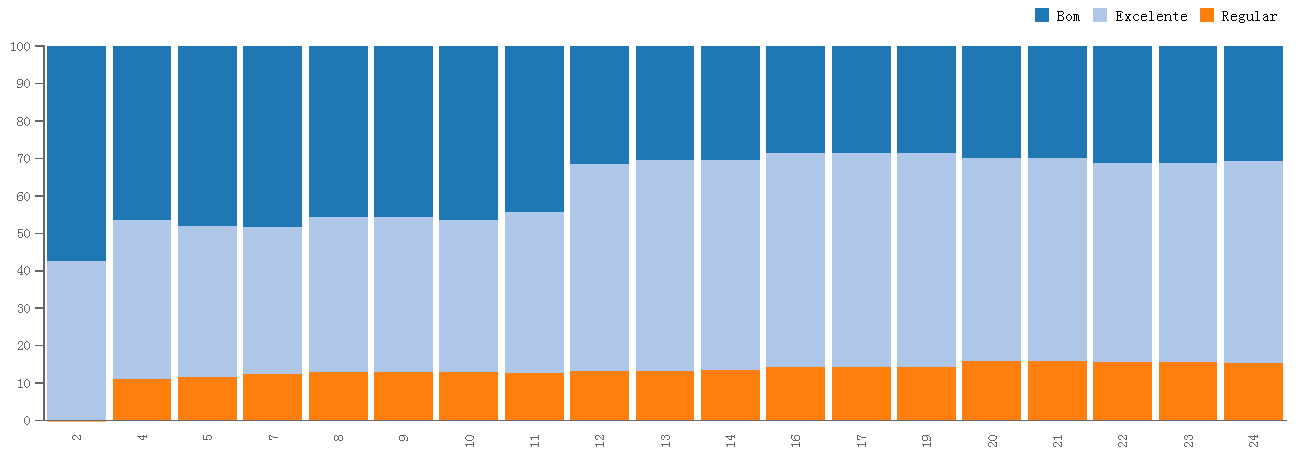
\includegraphics[scale=0.5]{figuras/todasmetricasSemCOB.png}
		\caption{Qualidade Geral das Métricas do Projeto SICG sem a CBO}
		\label{qualidadesprint}
\end{figure}

Enquanto a Figura \ref{qualidadesprint2} mostra a qualidade de todas as métricas analisadas ao longo das sprints do projeto considerando a métrica CBO. É possível perceber o grande impacto na qualidade geral do código fonte causado ao inserirmos na análise a métrica CBO. Ou seja, o código altamente acoplado e possuí uma quantidade alta de oportunidades de refatoração no que diz respeito aos seguintes cenários: classe pouco coesa, interface dos métodos, classes com muitos filhos, classe com métodos grandes e/ou muitos condicionais, classe com muita exposição e complexidade estrutural. 

\begin{figure}[H]
		\centering
			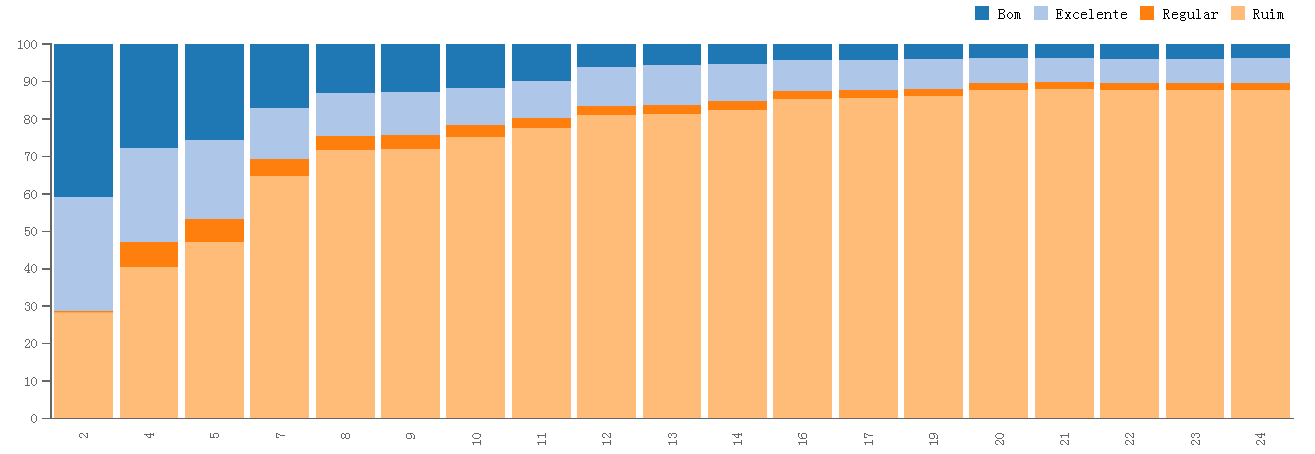
\includegraphics[scale=0.5]{figuras/todasmetricasComCOB.png}
		\caption{Qualidade Geral das Métricas do Projeto SICG com a CBO}
		\label{qualidadesprint2}
\end{figure}

A Figura \ref{cenarios} mostra qual a taxa de aproveitamento de oportunidade de limpeza por sprint. Ao analisarmos a última sprint do projeto, observamos que existe 43\%  da quantidade de classes do código fonte com oportunidades de refatoração. 

\begin{figure}[H]
		\centering
			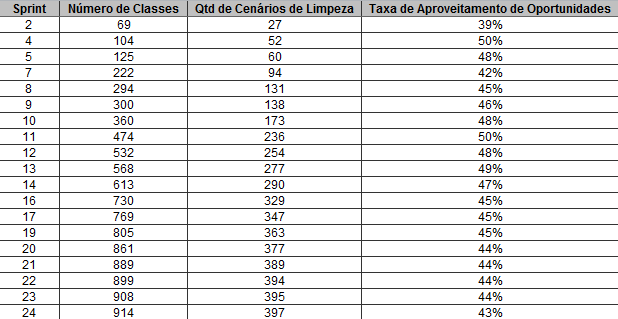
\includegraphics[scale=1.0]{figuras/cenarios.png}
		\caption{Cenários de Limpeza}
		\label{cenarios}
\end{figure}

A Figura \ref{percepcaoqualidade} mostra a percepção da qualidade do código fonte do SICG segundo os envolvidos no projeto (Scrum Master, Product Owner, Gestor do Contrato, Coordenador do Projeto, Fiscal Técnico e Desenvolvedores). Cerca de 66\% dos envolvidos consideraram  o intervalo de qualidade do código como "Excelente" e os demais consideraram
o intervalo de qualidade como "Bom".

\begin{figure}[H]
		\centering
			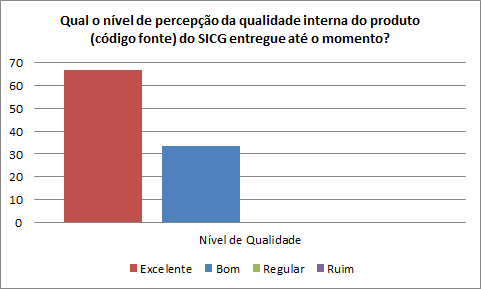
\includegraphics[scale=1.0]{figuras/percepcaoqualidade.png}
		\caption{Nível de Percepção da Qualidade do Código Fonte}
		\label{percepcaoqualidade}
\end{figure}

Assim, no que diz respeito a análise estática do código realizada, a qualidade do código fonte do projeto é satisfatória ao compararmos com o melhor software livre encontrado na linguagem de programação Java se considerarmos que a métrica COB não tem um peso relevante em comparação as demais métricas e também é satisfatória na percepção dos envolvidos no projeto SICG. No entanto, ao analisarmos que algumas das práticas ágeis adotadas tanto pela empresa quanto pelo órgão são refatoração, código limpo e revisão de código, o resultado obtido por este estudo de caso contradiz a percepção dos envolvidos.



